\documentclass[8pt]{beamer}
\usepackage[utf8]{inputenc}
\usepackage{xcolor}
\usepackage{colortbl}
\usepackage{epsfig}
% \usepackage{cancel}
\usepackage{ulem}
% \usepackage{threeparttable} % Joao Pela: 
\usepackage{amsmath}
\usepackage{hyperref}
% \usepackage{feynmp}         % For latex produced Feynman Diagrams

% Rule for feynmp diagrams to be considered graphics
% \DeclareGraphicsRule{*}{mps}{*}{}
% 
% % New compile sequence for feynmp
% \makeatletter
% \def\endfmffile{%
%   \fmfcmd{\p@rcent\space the end.^^J%
%           end.^^J%
%           endinput;}%
%   \if@fmfio
%     \immediate\closeout\@outfmf
%   \fi
%   \ifnum\pdfshellescape=\@ne
%     \immediate\write18{mpost \thefmffile}%
%   \fi}
% \makeatother

\usetheme{Madrid}

\author[João Pela]{J. Pela}
\title[]{MC VBF+MET QCD Samples Status}
\institute{Imperial College London}
\date{2014-02-01}

% The log drawn in the upper right corner.
\logo{\includegraphics[height=0.115\paperheight]{img/Logo_CMSICL.png}}

\begin{document}
\setlength{\unitlength}{1mm}

% ###################################################
\begin{frame}
  \titlepage
\end{frame}

% ###################################################
\begin{frame}{Today's presentation}
 
\begin{block}{Topics}
 
\begin{itemize}
  \item GenMET vs RecoMET study
  \begin{itemize}
    \item Fake MET contribution to QCD VBF samples
    \item GenMET filter optimization
  \end{itemize}
  \item First look at $\Delta\phi$ versus data
\end{itemize}
 
\end{block}
 
\end{frame}

% ###################################################
\begin{frame}{Fake met contribution study}
 
To evaluate how much events pass out analysis cut of $MET>130$ $GeV$ that have a significant contribution of fake MET 
which the new QCD VBF-like samples will not be able to simulate we need to look at the inclusive samples.

\begin{columns}
 
\column[t]{0.45\linewidth}  
\begin{block}{Area Definition}
 
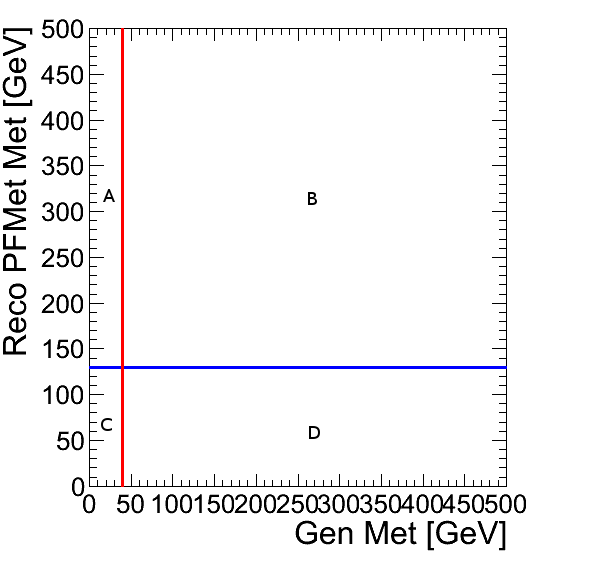
\includegraphics[width=\linewidth]{img/basic.png}
 
\end{block}

\column[t]{0.45\linewidth}  
\begin{block}
 
We can define 4 areas:
\begin{itemize}
 \item A: Accepted by Analysis MET cut but rejected by GenMET Filter
 \item B: Accepted by Analysis MET cut and accepted by GenMET Filter
 \item C: Rejected by Analysis MET cut and rejected by GenMET Filter
 \item D: Rejected by Analysis MET cut but accepted by GenMET Filter
\end{itemize}

From this we can define the B area normalization factor as $\frac{A+B}{B}$

\end{block}

\end{columns}

\end{frame}

% ###################################################
\begin{frame}{Gen Met Vs Reco MET I}

Plots here do now have any weighting but cross section since filters will operate over genEvents with no weigting this (so this is just a scaling).

\begin{columns}
    
\column[t]{0.45\linewidth}  
\begin{block}{80to120}
 
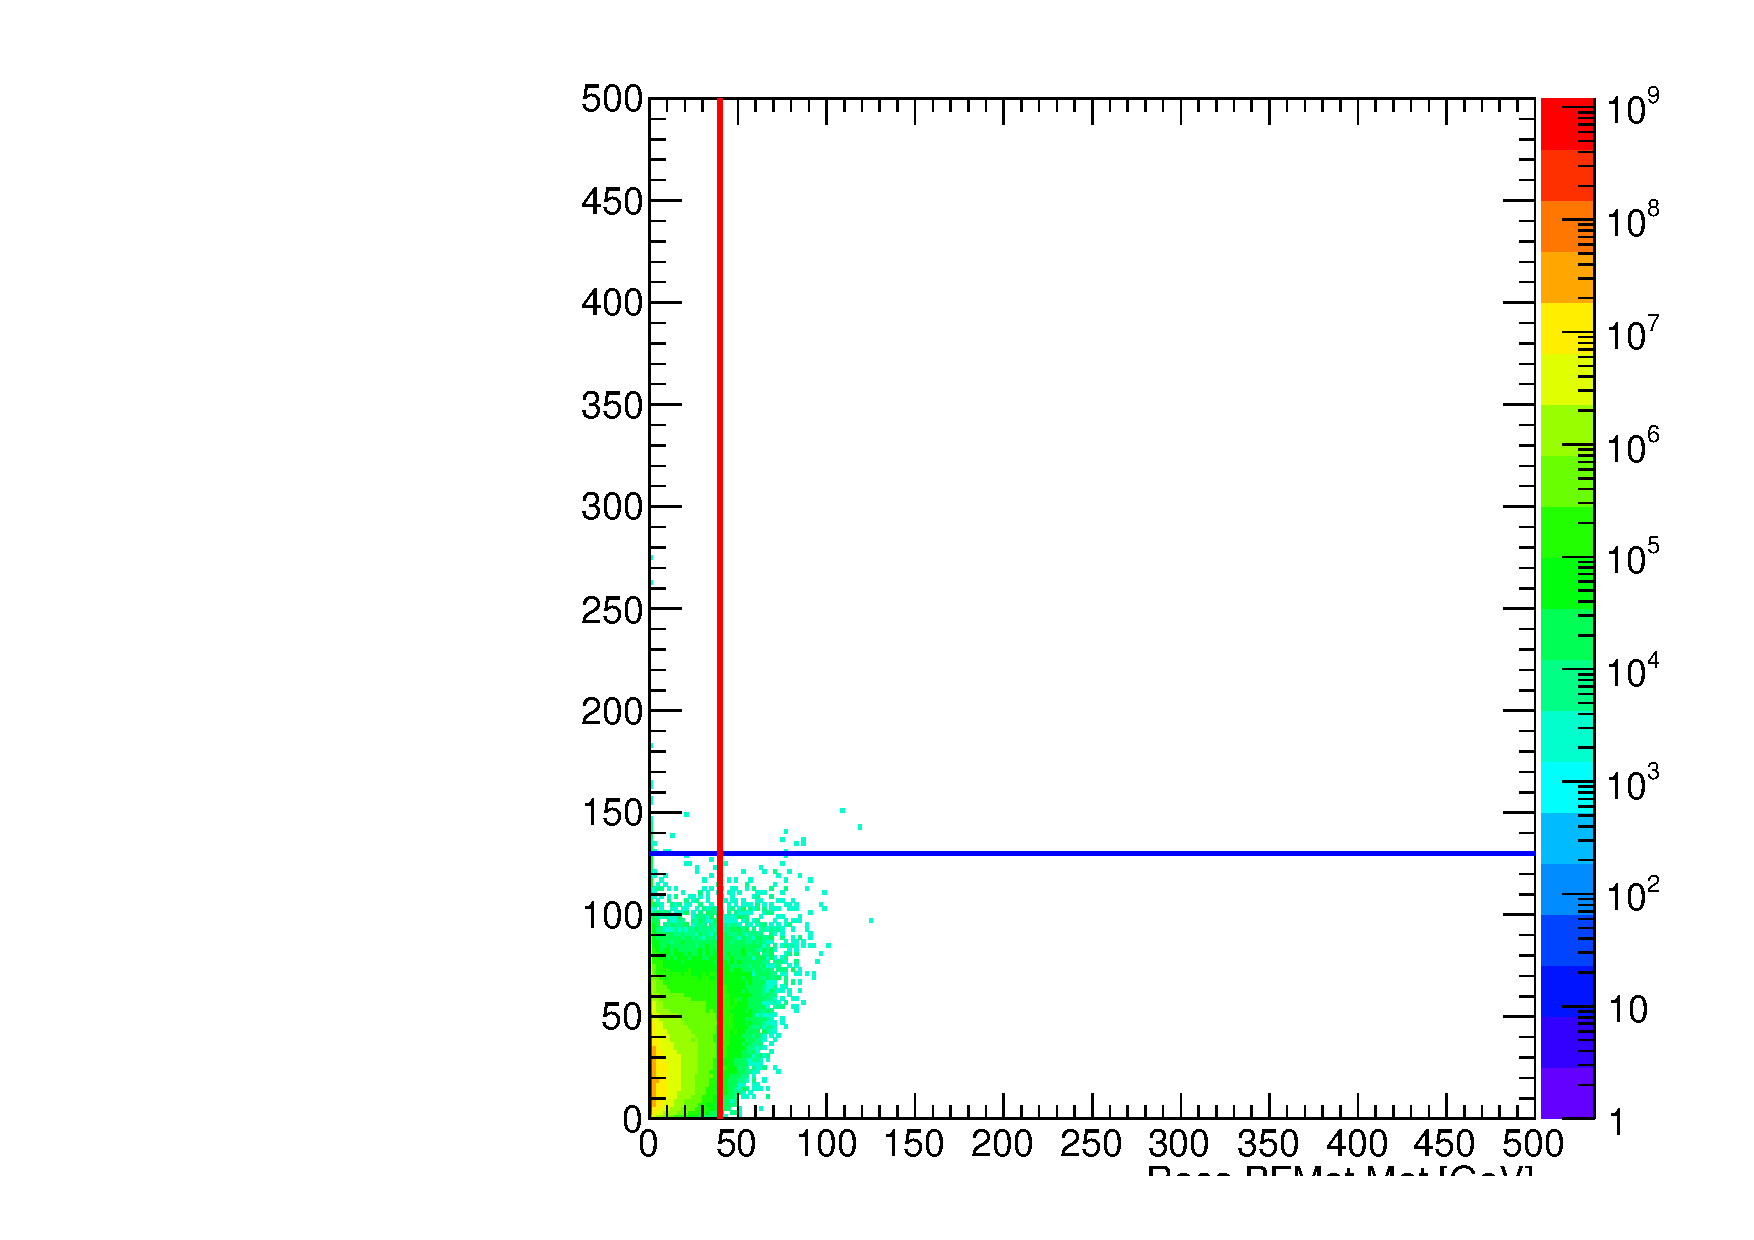
\includegraphics[width=\linewidth]{img/MC_QCD-Pt-80to120-pythia6_GenVsReco_met}

\end{block}

\column[t]{0.45\linewidth}  
\begin{block}{120to170}
 
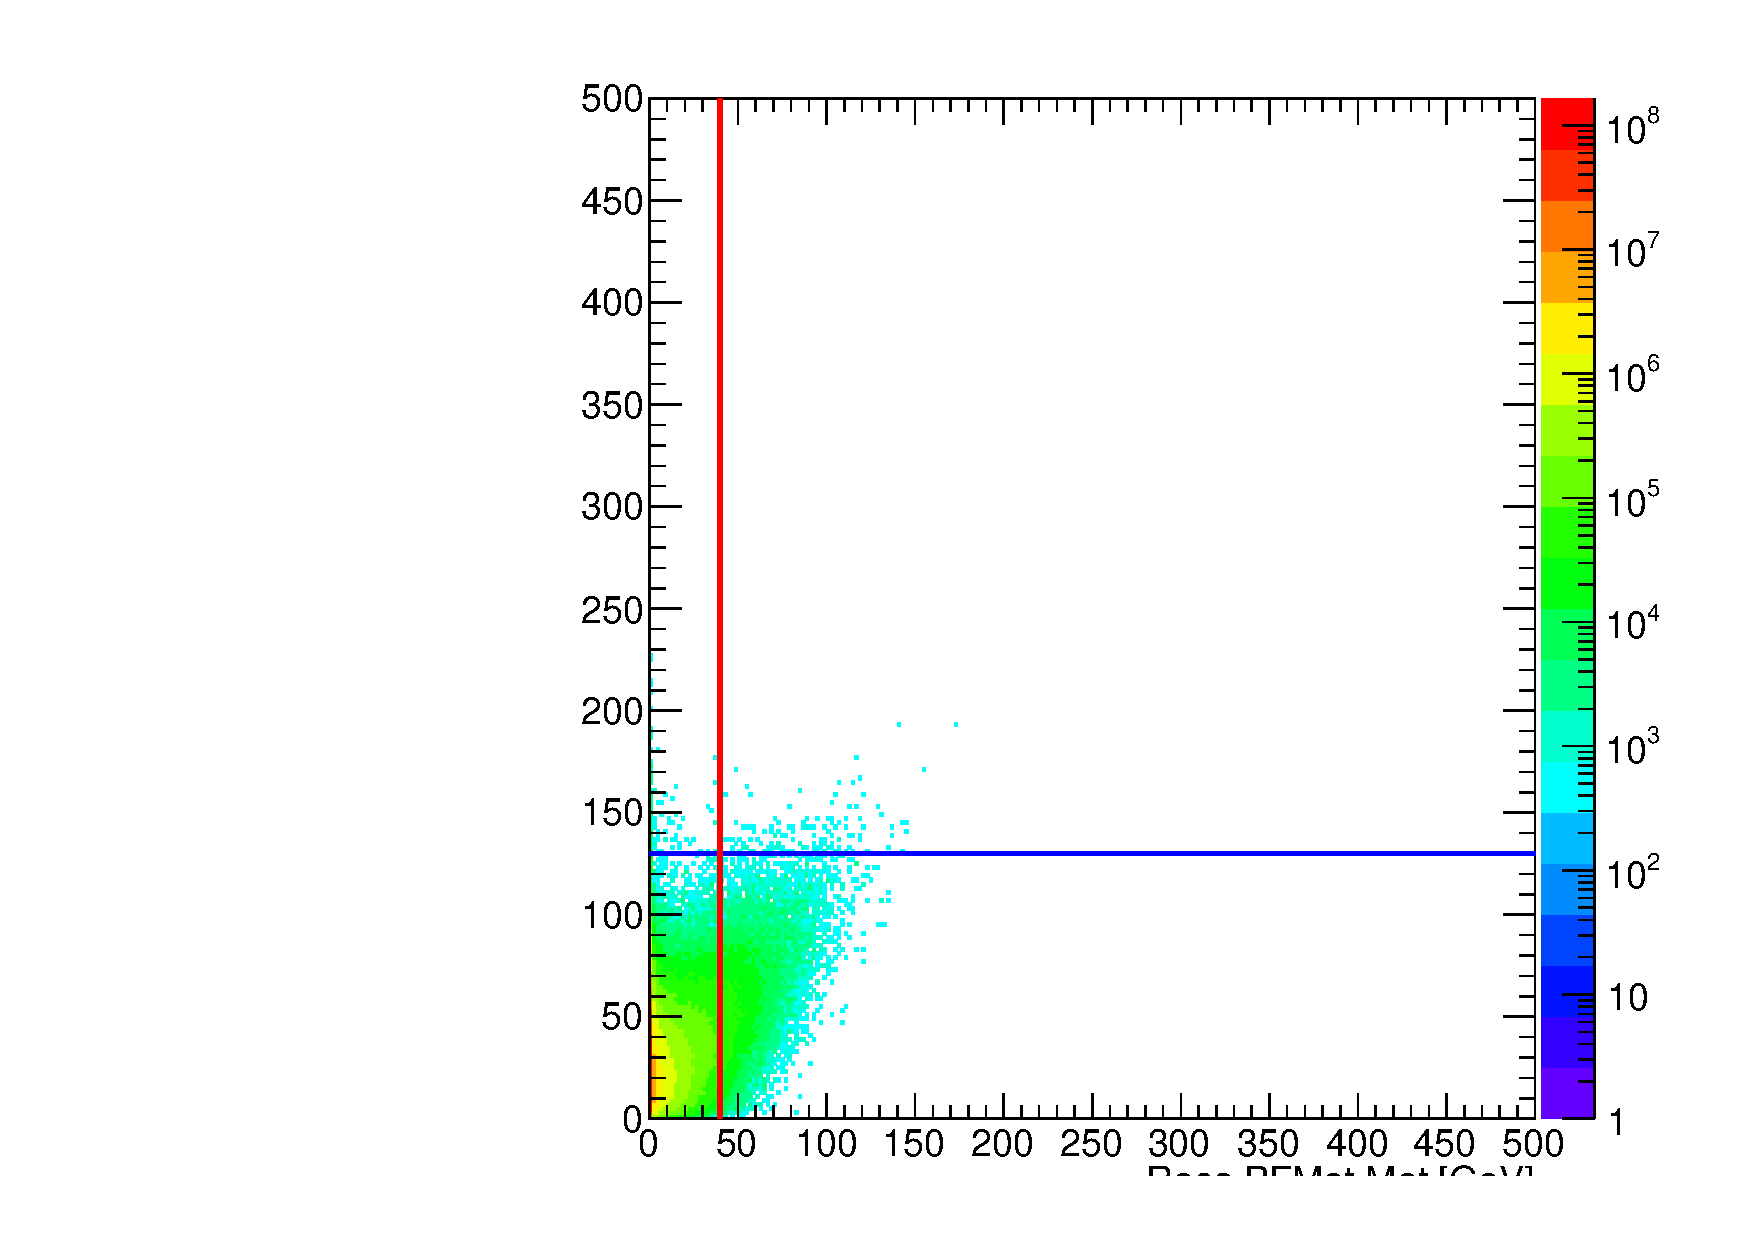
\includegraphics[width=\linewidth]{img/MC_QCD-Pt-120to170-pythia6_GenVsReco_met}

\end{block}

\end{columns}

For both this $p_T$ hats most event fall on zone C or D and are rejected analysis cut.

\end{frame}

% ###################################################
\begin{frame}{Gen Met Vs Reco MET II}

Plots here do now have any weighting but cross section since filters will operate over genEvents with no weigting this (so this is just a scaling).

\begin{columns}

\column[t]{0.45\linewidth}  
\begin{block}{170to300}
 
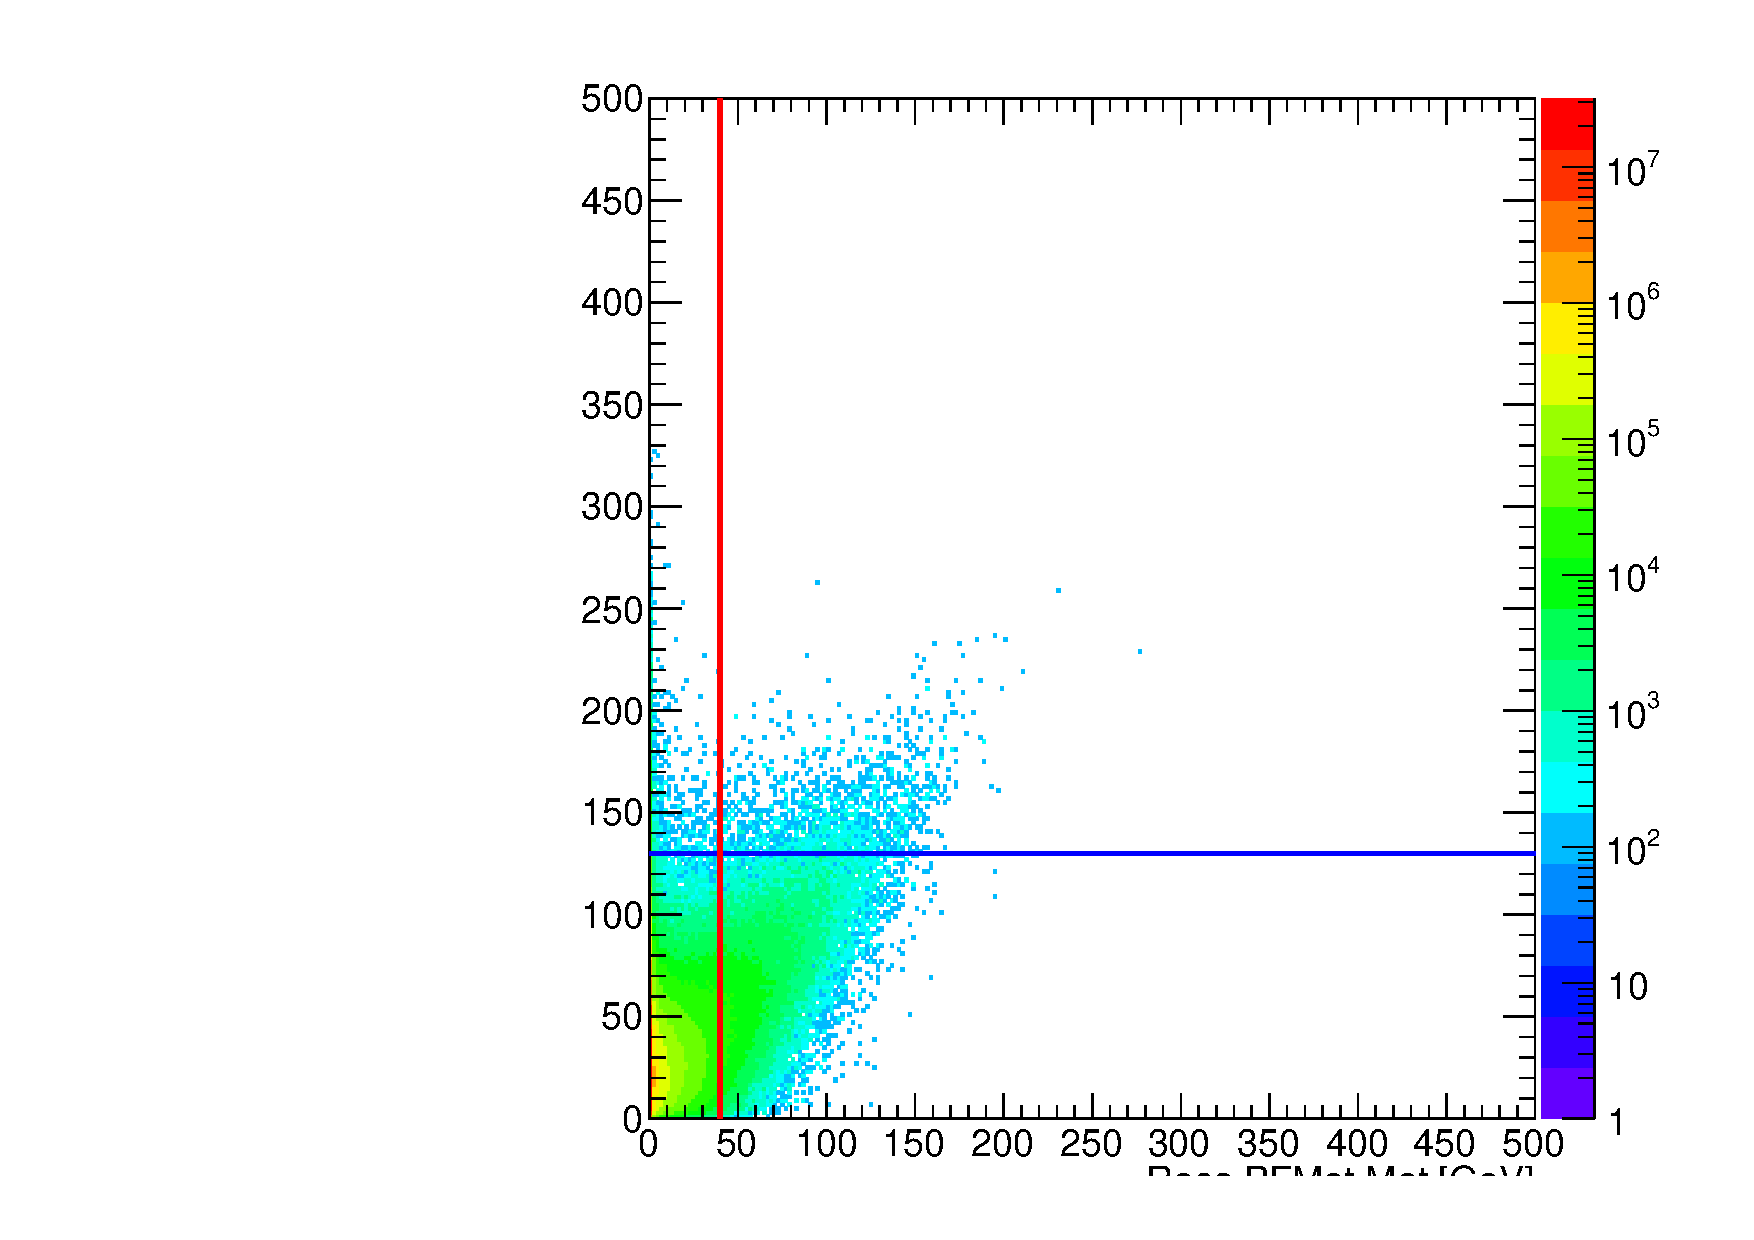
\includegraphics[width=\linewidth]{img/MC_QCD-Pt-170to300-pythia6_GenVsReco_met}
 
\end{block}


\column[t]{0.45\linewidth}  
\begin{block}{300to470}
 
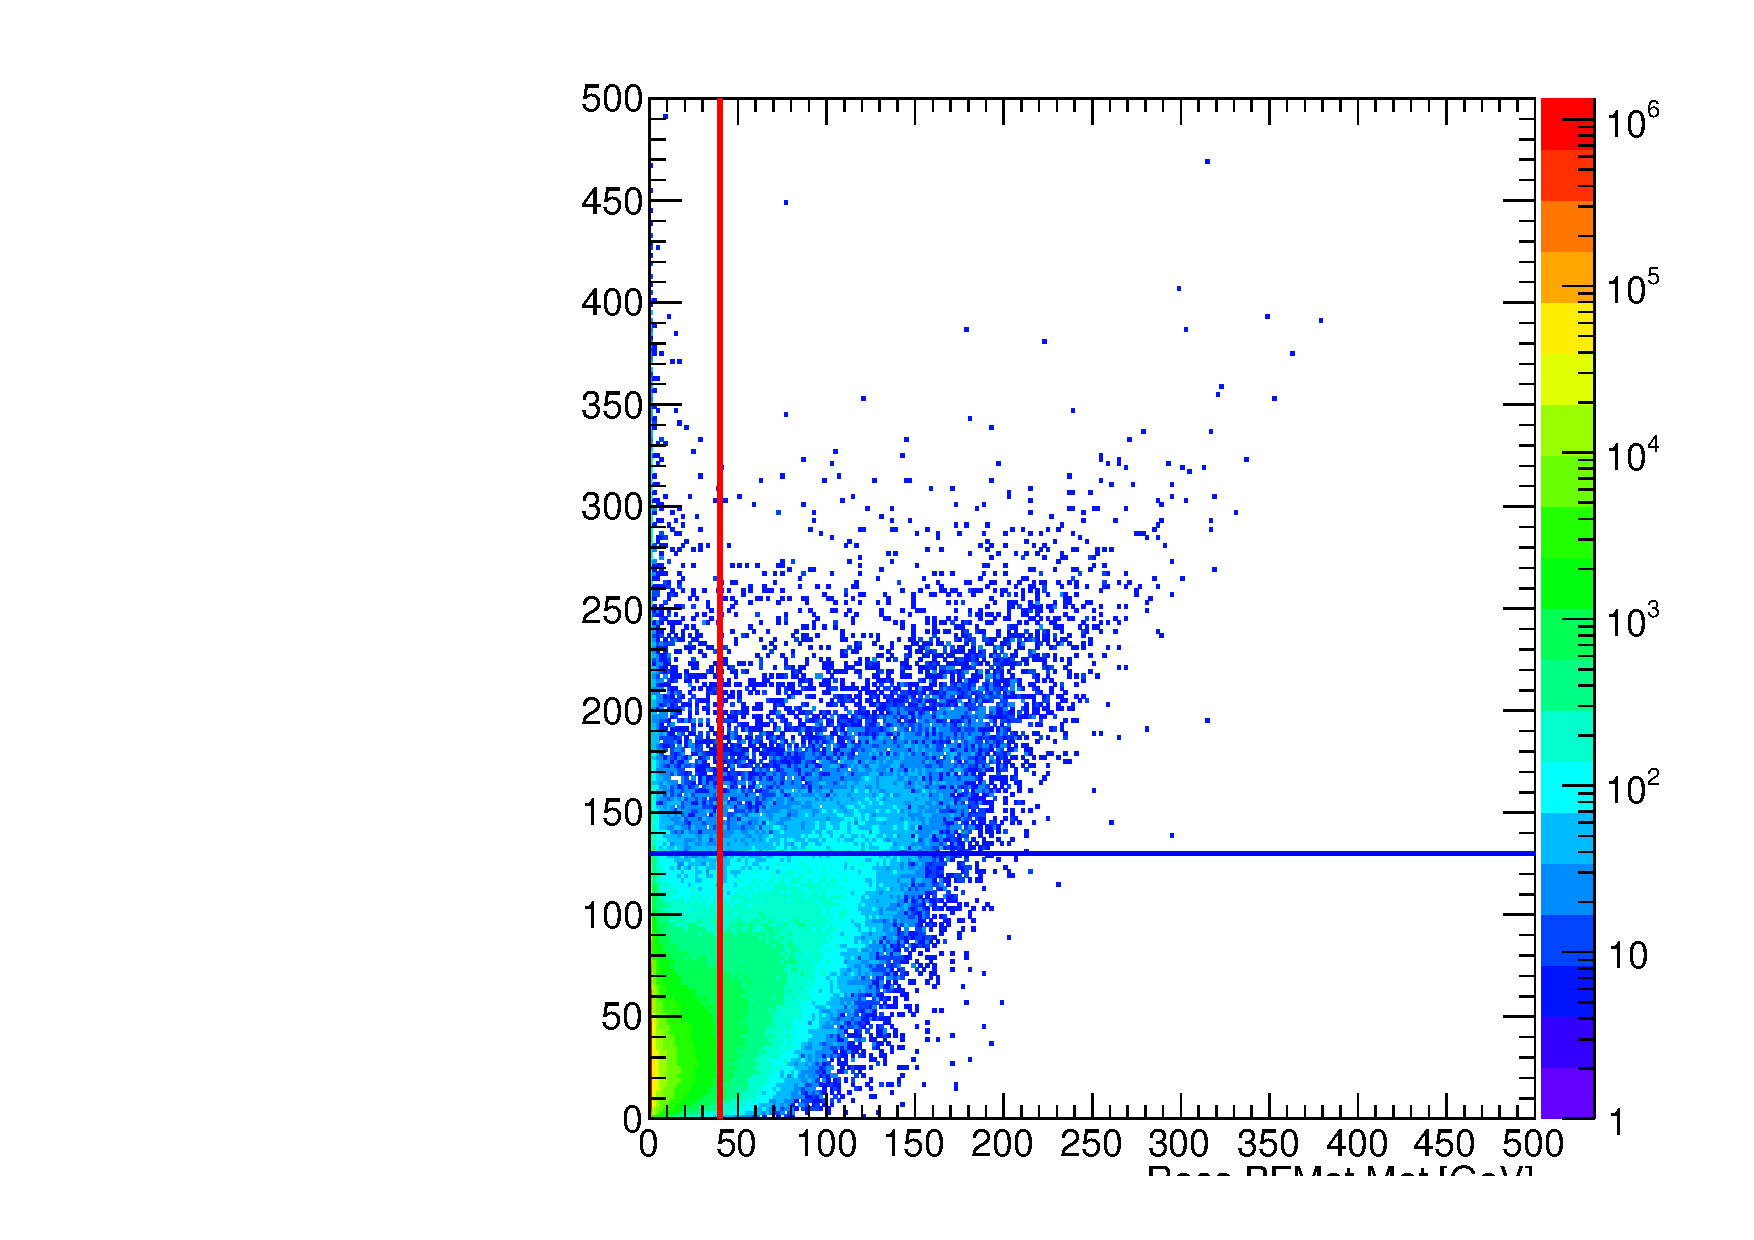
\includegraphics[width=\linewidth]{img/MC_QCD-Pt-300to470-pythia6_GenVsReco_met}

\end{block}

\end{columns}

We can se for this $p_T$ hats a significant population of events now in areas A and B.

\end{frame}

% ###################################################
\begin{frame}{Gen Met Vs Reco MET III}

Plots here do now have any weighting but cross section since filters will operate over genEvents with no weigting this (so this is just a scaling).
Plot on the right Adds all the QCD inclusive $p_T$ hats taking into account the relative cross section.

\begin{columns}

\column[t]{0.45\linewidth}  
\begin{block}{470to600}
 
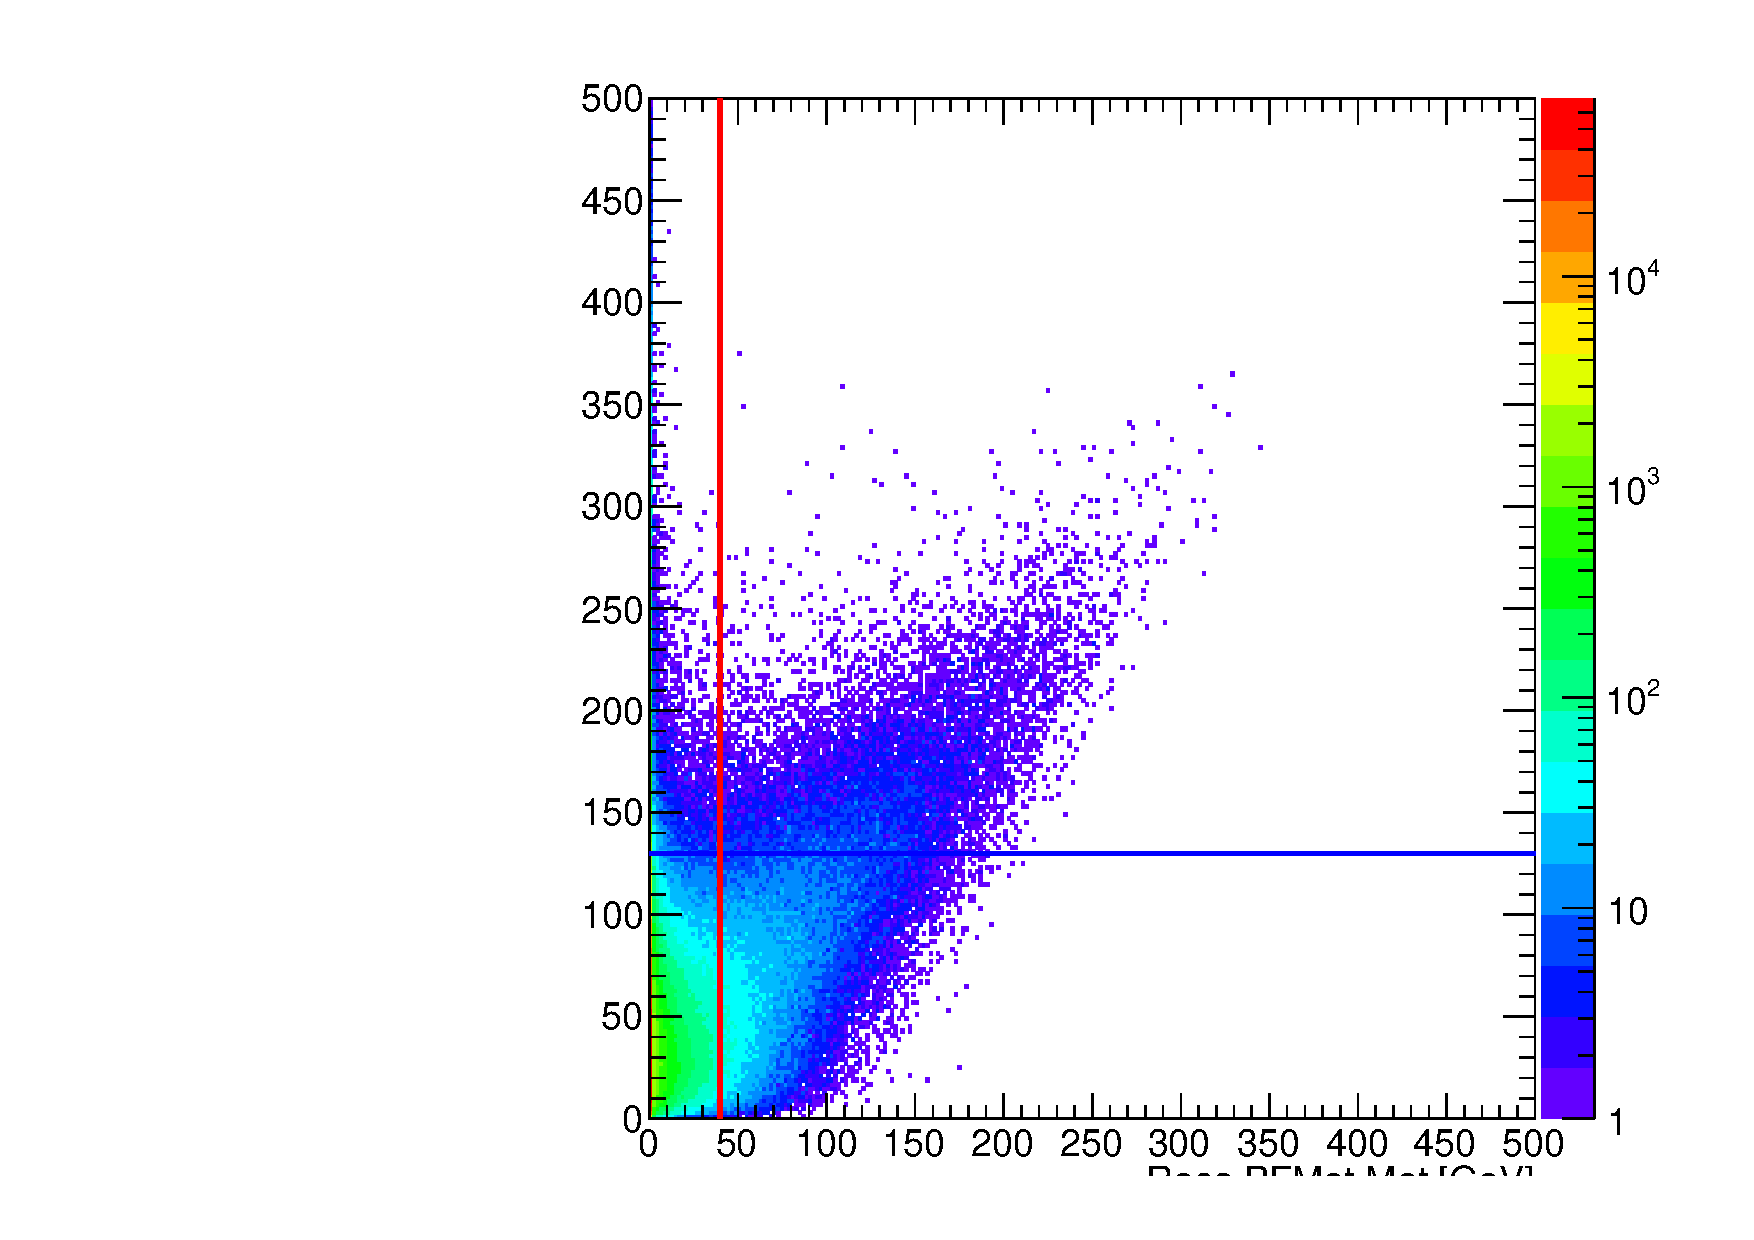
\includegraphics[width=\linewidth]{img/MC_QCD-Pt-470to600-pythia6_GenVsReco_met}

\end{block}

\column[t]{0.45\linewidth}  
\begin{block}{Total}
 
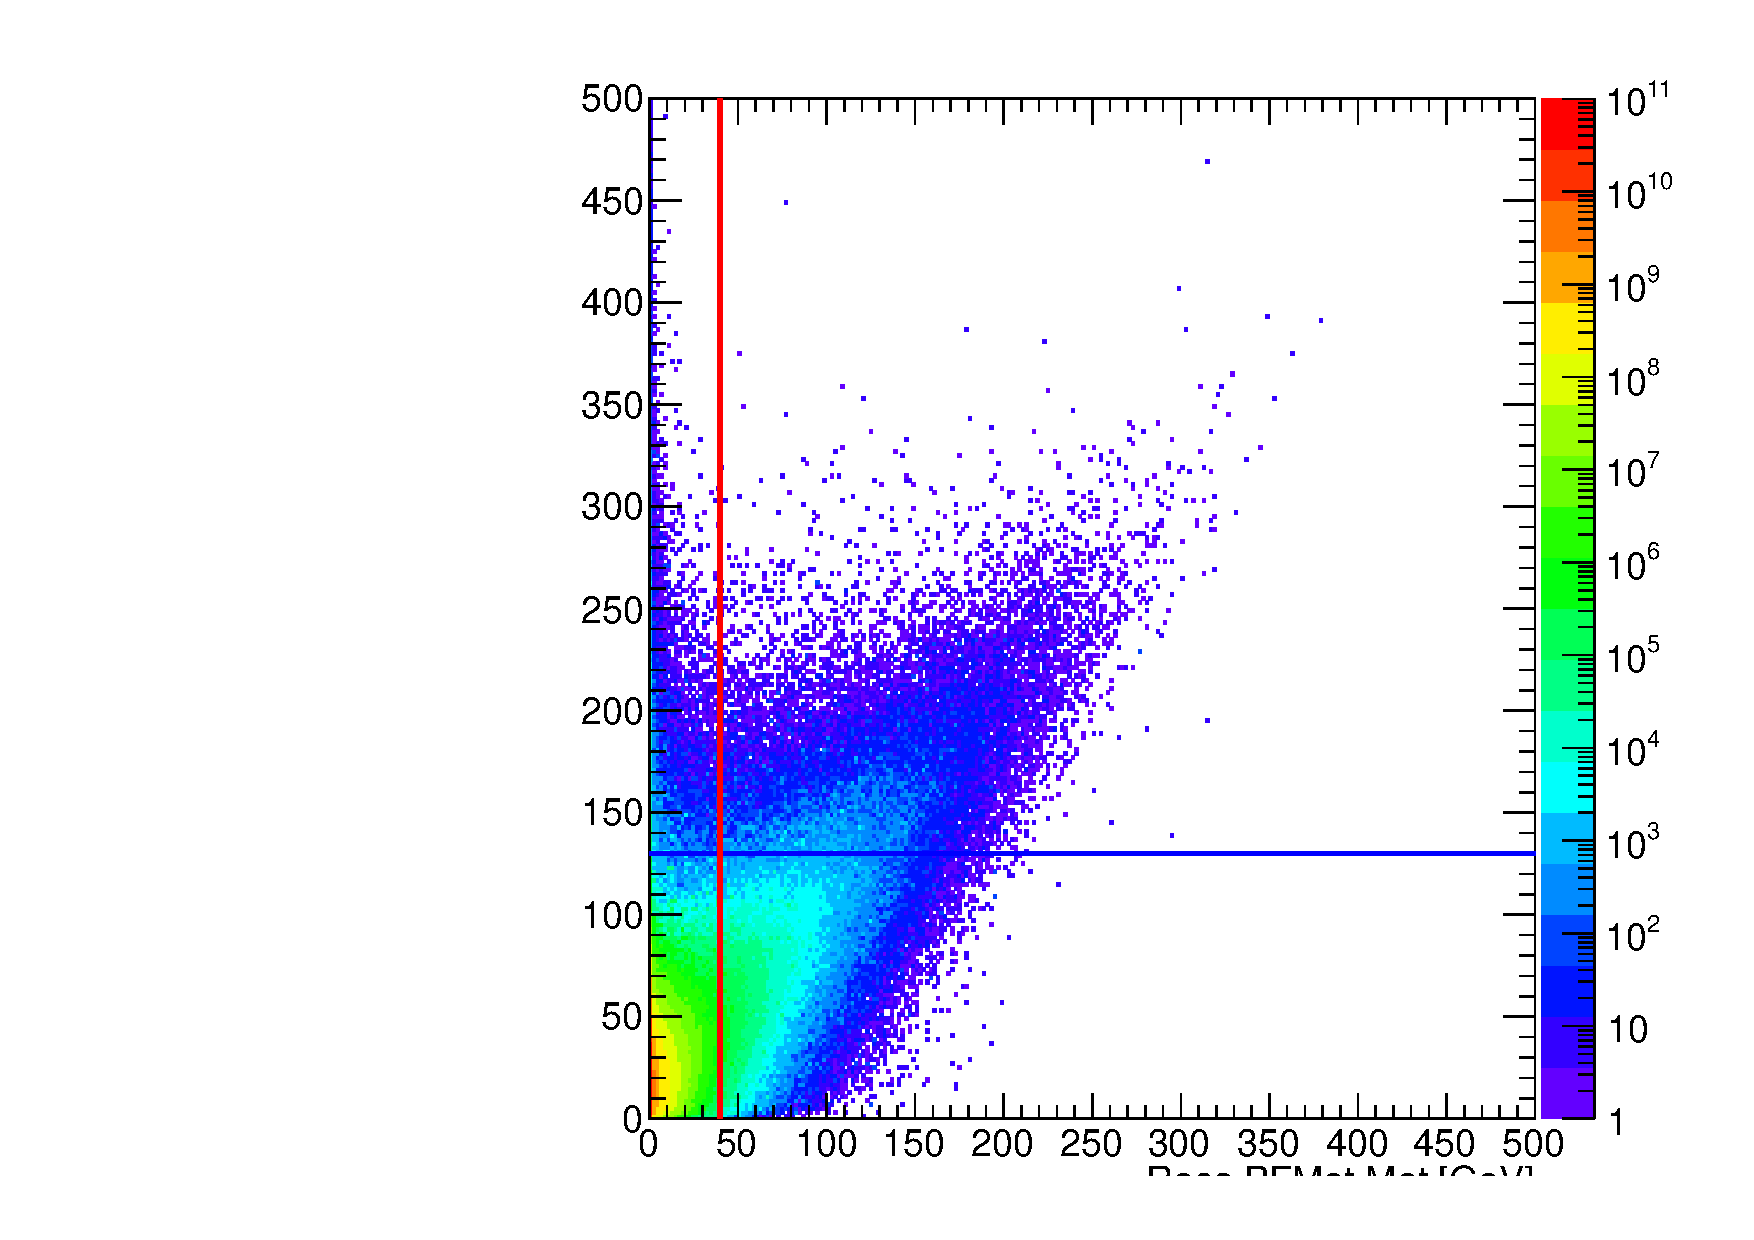
\includegraphics[width=\linewidth]{img/MC_QCDIncAll_GenVsReco_met}
 
\end{block}

\end{columns}

We can see in both plots that there is a significant population in both areas A and B.

\end{frame}

% ###################################################
\begin{frame}{Gen Met Vs Reco MET - Into Numbers}

Now we can calculate what is the percentage of events in each area and the normalization factor for B are.

\begin{block}{Areas and normalization factor}

\begin{table}[!h]
\centering
\resizebox{\linewidth}{!}{
\begin{tabular}{|c||c|c|c|c||c|}
\hline
Sample & A & B & C & D & Factor \\
\hline \hline
MC\_QCD-Pt-30to50-pythia6 & 0.000000 & 0.000000 & 0.999997 & 0.000003 & inf \\
MC\_QCD-Pt-50to80-pythia6 & 0.000000 & 0.000000 & 0.999884 & 0.000116 & nan \\
MC\_QCD-Pt-80to120-pythia6 & 0.000006 & 0.000001 & 0.998800 & 0.001193 & 5.625 \\
MC\_QCD-Pt-120to170-pythia6 & 0.000065 & 0.000024 & 0.995715 & 0.004195 & 3.676 \\
MC\_QCD-Pt-170to300-pythia6 & 0.000684 & 0.000281 & 0.989966 & 0.009069 & 3.432 \\
MC\_QCD-Pt-300to470-pythia6 & 0.005185 & 0.002331 & 0.976764 & 0.015721 & 3.224 \\
MC\_QCD-Pt-470to600-pythia6 & 0.016652 & 0.005900 & 0.959474 & 0.017973 & 3.823 \\
MC\_QCD-Pt-600to800-pythia6 & 0.034093 & 0.008591 & 0.939409 & 0.017906 & 4.969 \\
MC\_QCD-Pt-800to1000-pythia6 & 0.068863 & 0.011177 & 0.903115 & 0.016845 & 7.161 \\
MC\_QCD-Pt-1000to1400-pythia6 & 0.117719 & 0.012717 & 0.854500 & 0.015063 & 10.257 \\
MC\_QCD-Pt-1400to1800-pythia6 & 0.202556 & 0.014259 & 0.770444 & 0.012741 & 15.206 \\
MC\_QCD-Pt-1800-pythia6 & 0.285060 & 0.015070 & 0.688829 & 0.011041 & 19.916 \\
\hline \hline
Total & 0.000001 & 0.000000 & 0.999954 & 0.000044 & 4.761343 \\
\hline
\end{tabular}

}
\caption{Relative are for A, B, C and D areas and factor to normalize B area to A+B (normalize QCD VBF samples to inclusive at $MET>130$ $GeV$ cut.}
\end{table}

\end{block}

The normalization factors seem to be approximatly of the order of the discrepancy in yields seen last week.

\end{frame}

% ###################################################
\begin{frame}{Aplying Factors to last week tables}

Considerations
\begin{itemize}
  \item Factors are calculated for uncorrected (PU, Trigger and ID) events and applied to tables from last week which
        is to some level \uline{wrong} but at first approximation gives an idea of the effect of this normalization factors.
  \item Factors only acount for events lost due to fake MET which is just one of the 2 filters applied, the VBF QCD jets filters
        while have its own losses which need to be accounted in parallel.
\end{itemize}

\begin{block}{Correcting a MET cut level}

\resizebox{\linewidth}{!}{
\begin{tabular}{|c||cc||cc||cc||cc||cc|}
\hline
 & 80-120 & 80-120 & 120-170 & 120-170 & 170-300 & 170-300 & 300-470 & 300-470 & 470-600 & 470-600 \\
\hline
Cut                & Inc  &     VBF &     Inc &     VBF &     Inc &     VBF &    Inc &    VBF &  Inc & VBF \\
\hline \hline
MET (Last Week)    & 1.50 &  300.35 & 4672.18 &  682.16 & 3577.84 &  661.70 & 232.67 &  43.28 & 4.06 & 0.82 \\
MET (Apply factor) & 1.50 & 1689.46 & 4672.18 & 2507.62 & 3577.84 & 2270.95 & 232.67 & 139.53 & 4.06 & 3.13 \\
\hline
\end{tabular}
}

\end{block}

Number are now much closer to match, execept on the 80-120 $GeV$ bin where QCD inclusive only has one event highly suppressed but non xsec weights. 
Note bin 470-600 $GeV$ where both QCD Inc and QCD VBF have enough statistics to simulate 20 $fb^{-1}$ now are much closer.


\end{frame}

% ###################################################
\begin{frame}{DPhi compared with Data}
 
Both plots are normalized to 1 to observe shapes.
 
\begin{columns}
 
\column[t]{0.45\linewidth}  
\begin{block}{At Tight $M_{jj}$ level}
 
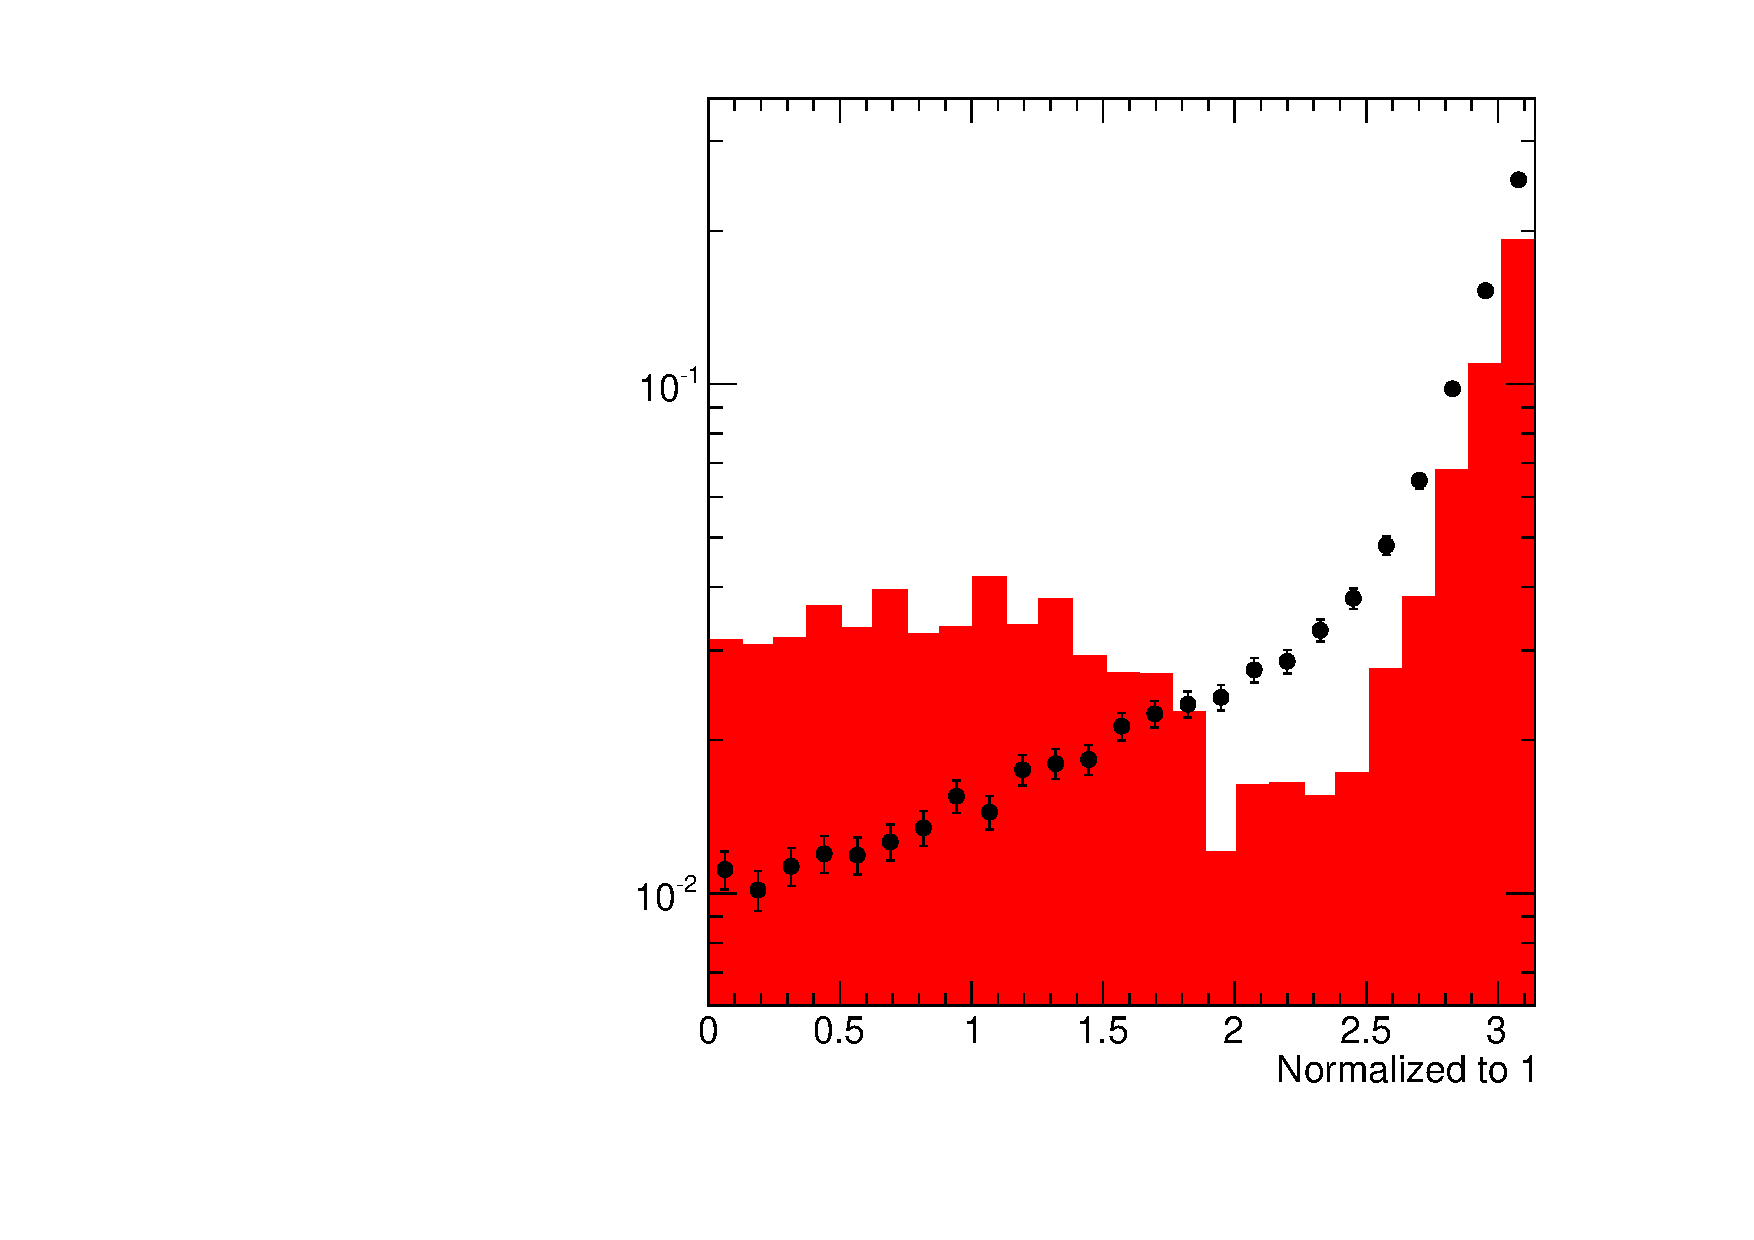
\includegraphics[width=\linewidth]{img/DataVsQCDVBF_TightMjj_dphijj}
 
\end{block}
 
\column[t]{0.45\linewidth}  
\begin{block}{CJV level}

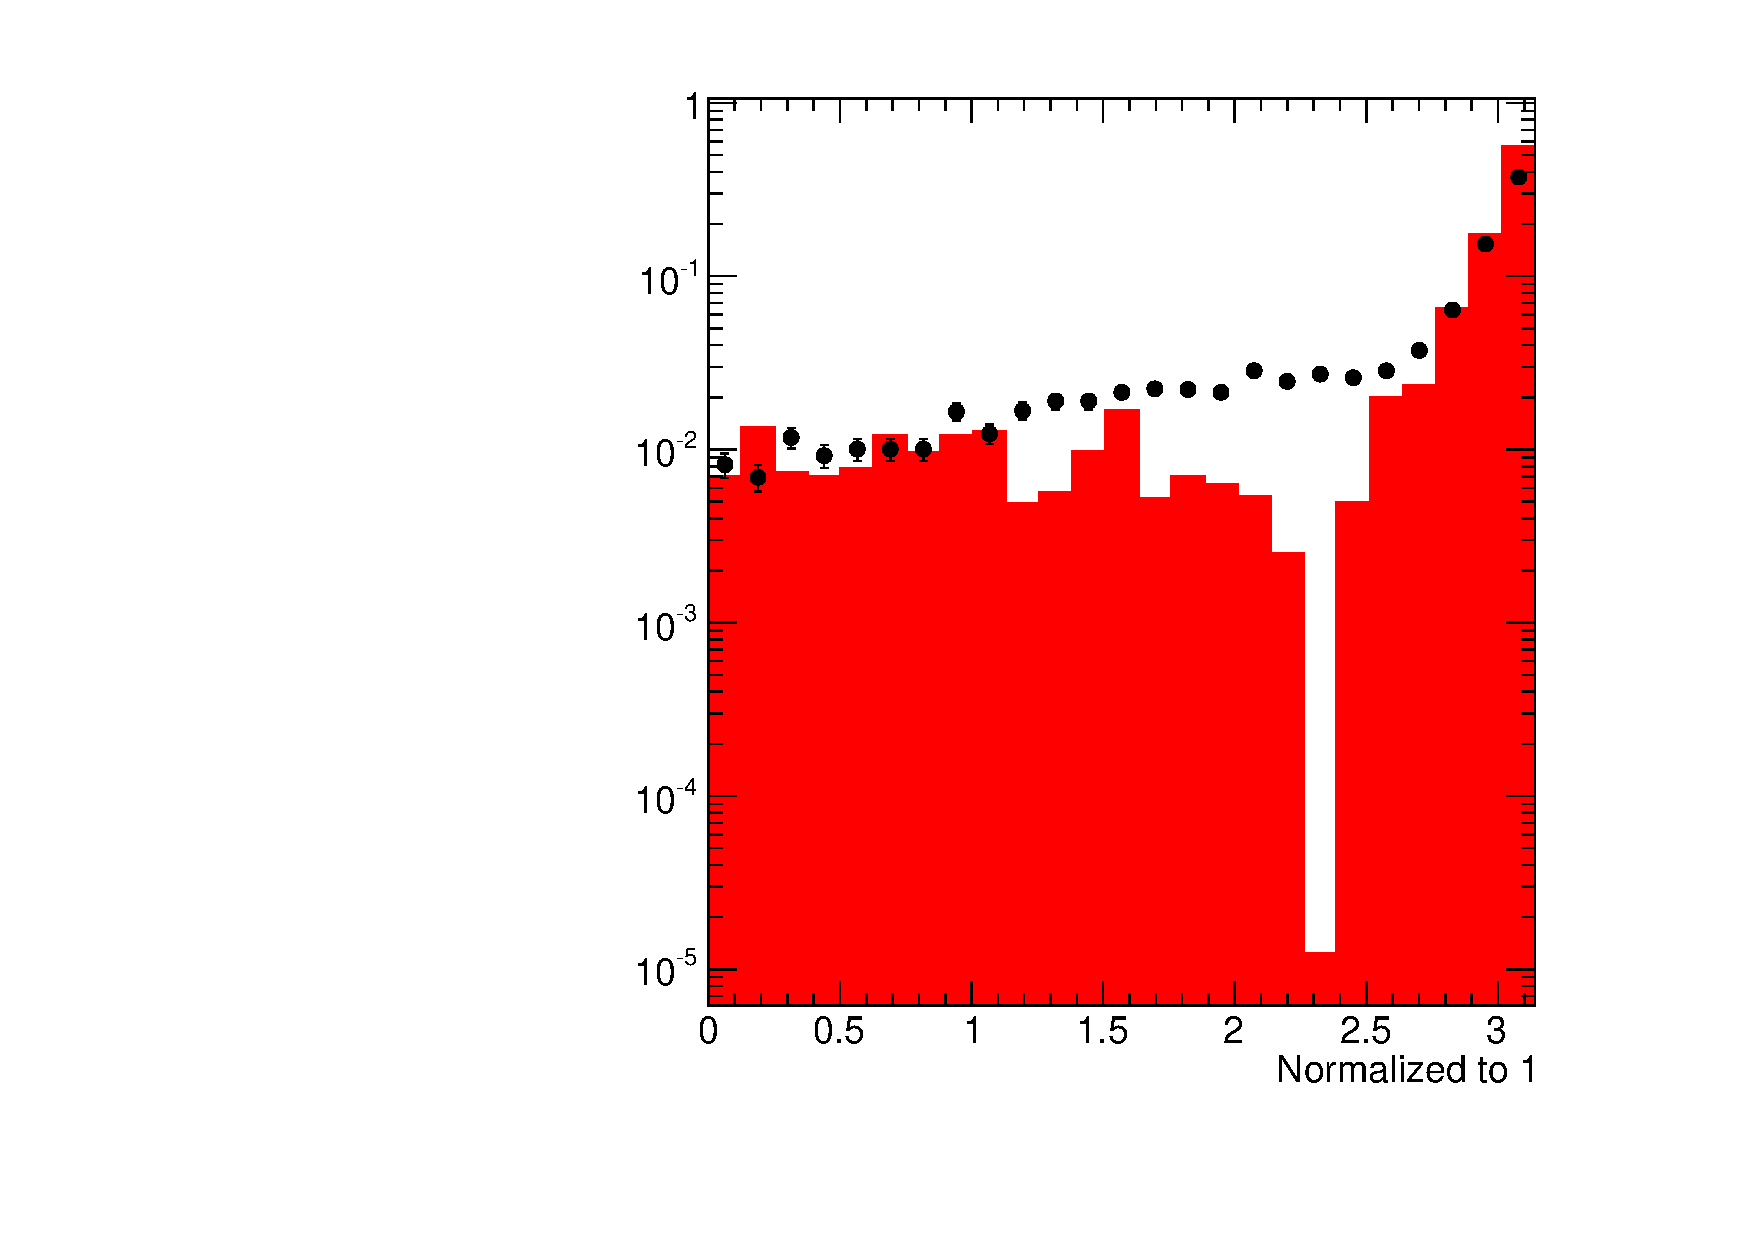
\includegraphics[width=\linewidth]{img/DataVsQCDVBF_CJVpass_dphijj}
 
\end{block}

\end{columns}

It is interesting to notice that while shapes do not match very well are Tight $m_{jj}$ they match ``well'' at CJV level including at low values except for dphi around 2.3.

\end{frame}

\end{document}